\documentclass[aspectratio=169,x11names]{beamer}
\usetheme{Pittsburgh}
\usepackage{xcolor}
\usepackage[utf8]{inputenc}
\usepackage[german]{babel}
\usepackage{amsmath}
\usepackage{amsfonts}
\usepackage{amssymb}
\usepackage{graphicx}
\usepackage{multicol}
\usepackage{wrapfig}
\usepackage{hyperref}

\author{Jonas Betzendahl}
\title{Machine Learning Science Slam}

\beamertemplatenavigationsymbolsempty 

% For Footnotes without markers on the slide
% https://tex.stackexchange.com/questions/30720/footnote-without-a-marker
\newcommand\blfootnote[1]{%
  \begingroup
  \renewcommand\thefootnote{}\footnote{#1}%
  \addtocounter{footnote}{-1}%
  \endgroup
}

%src: https://tex.stackexchange.com/questions/34921/how-to-overlap-images-in-a-beamer-slide
\def\Put(#1,#2)#3{\leavevmode\makebox(0,0){\put(#1,#2){#3}}}

\begin{document}

%------------------------------------------------------------------------------------
\section{Introduction}

\begin{frame}
\begin{center}
\vfill
\huge Maschinelles Lernen
\normalsize 

(Und warum das vielleicht gruseliger ist, als es klingt)
\bigskip\bigskip

\large Jonas Betzendahl, M.Sc.
\bigskip\bigskip

\href{https://twitter.com/lambdatotoro}{
\includegraphics[scale=0.125]{images/twitter_logo.png}}
\href{https://chaos.social/@lambdatotoro}{\includegraphics[scale=0.125]{images/mastodon_logo.png}}
\href{https://github.com/jbetzend}{
\includegraphics[scale=0.125]{images/github_logo.png}}
\href{https://whispeer.de/en/user/jbetzend}{
\includegraphics[scale=0.125]{images/whispeer_logo.png}}

\texttt{@lambdaTotoro (@chaos.social)}
\end{center}
\end{frame}


%------------------------------------------------------------------------------------

\begin{frame}
\frametitle{Small Talk in Intelligent Systems}

\begin{multicols}{2}

Mein Studium: \glqq Intelligente Systeme\grqq .

Was war wohl die häufigste Frage an meinen Studiengang?

\pause

\begin{center}
\glqq Na, wie lange dauert\\ es noch bis zur\\ Roboterapokalypse?\grqq
\end{center}

\columnbreak

\begin{center}

\includegraphics[height=0.7\textheight,keepaspectratio]{images/mtt.png} 
\end{center}
\end{multicols}
\end{frame}

\begin{frame}
\begin{center}

\includegraphics[width=\textwidth]{images/amazon-logo.jpg} 
\end{center}
\end{frame}

\begin{frame}
\begin{center}

\includegraphics[width=\textwidth]{images/amazon-one-wallet.jpg} 
\end{center}
\end{frame}

\begin{frame}
\begin{center}
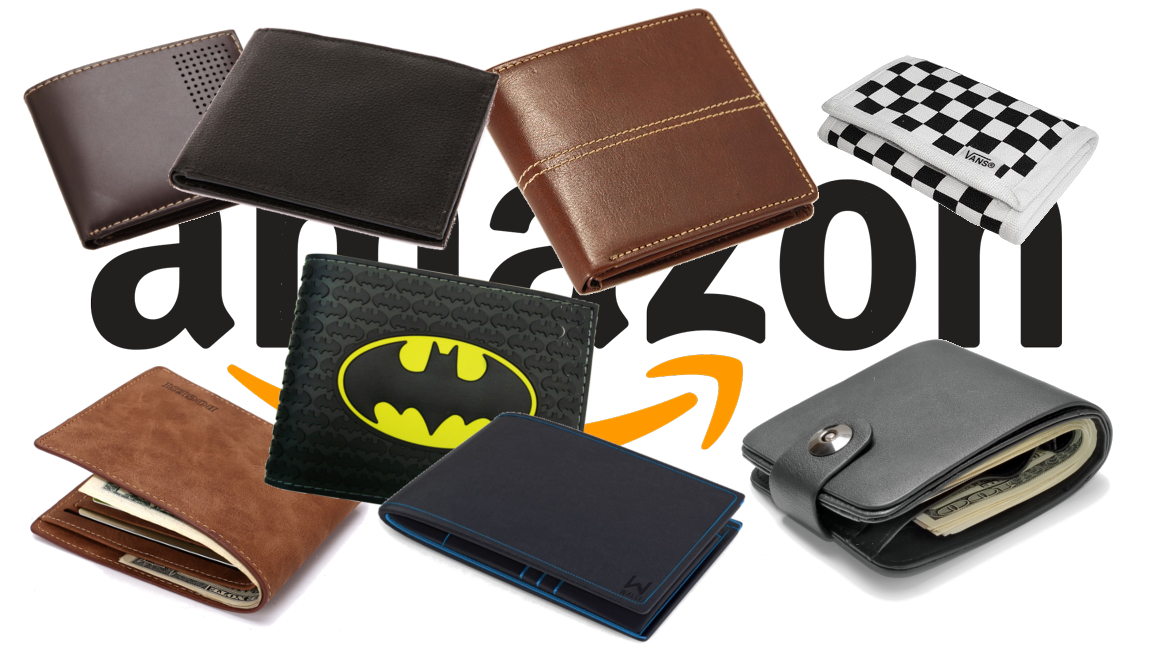
\includegraphics[width=\textwidth]{images/amazon-buncha-wallets.jpg} 
\end{center}
\end{frame}

%------------------------------------------------------------------------------------

\begin{frame}

\begin{center}
\dots zumindest habe ich bisher so immer meine Slams angefangen.
\bigskip

Wir müssen reden!
\end{center}

\end{frame}

\section{Die Vorteile von Maschinellem Lernen}

\begin{frame}
\begin{center}
\huge
Die Errungenschaften\\von Maschinellem Lernen
\end{center}
\end{frame}

\begin{frame}

\begin{center}
Maschinelles Lernen ist mächtig und nützlich\dots
\end{center}

\begin{center}
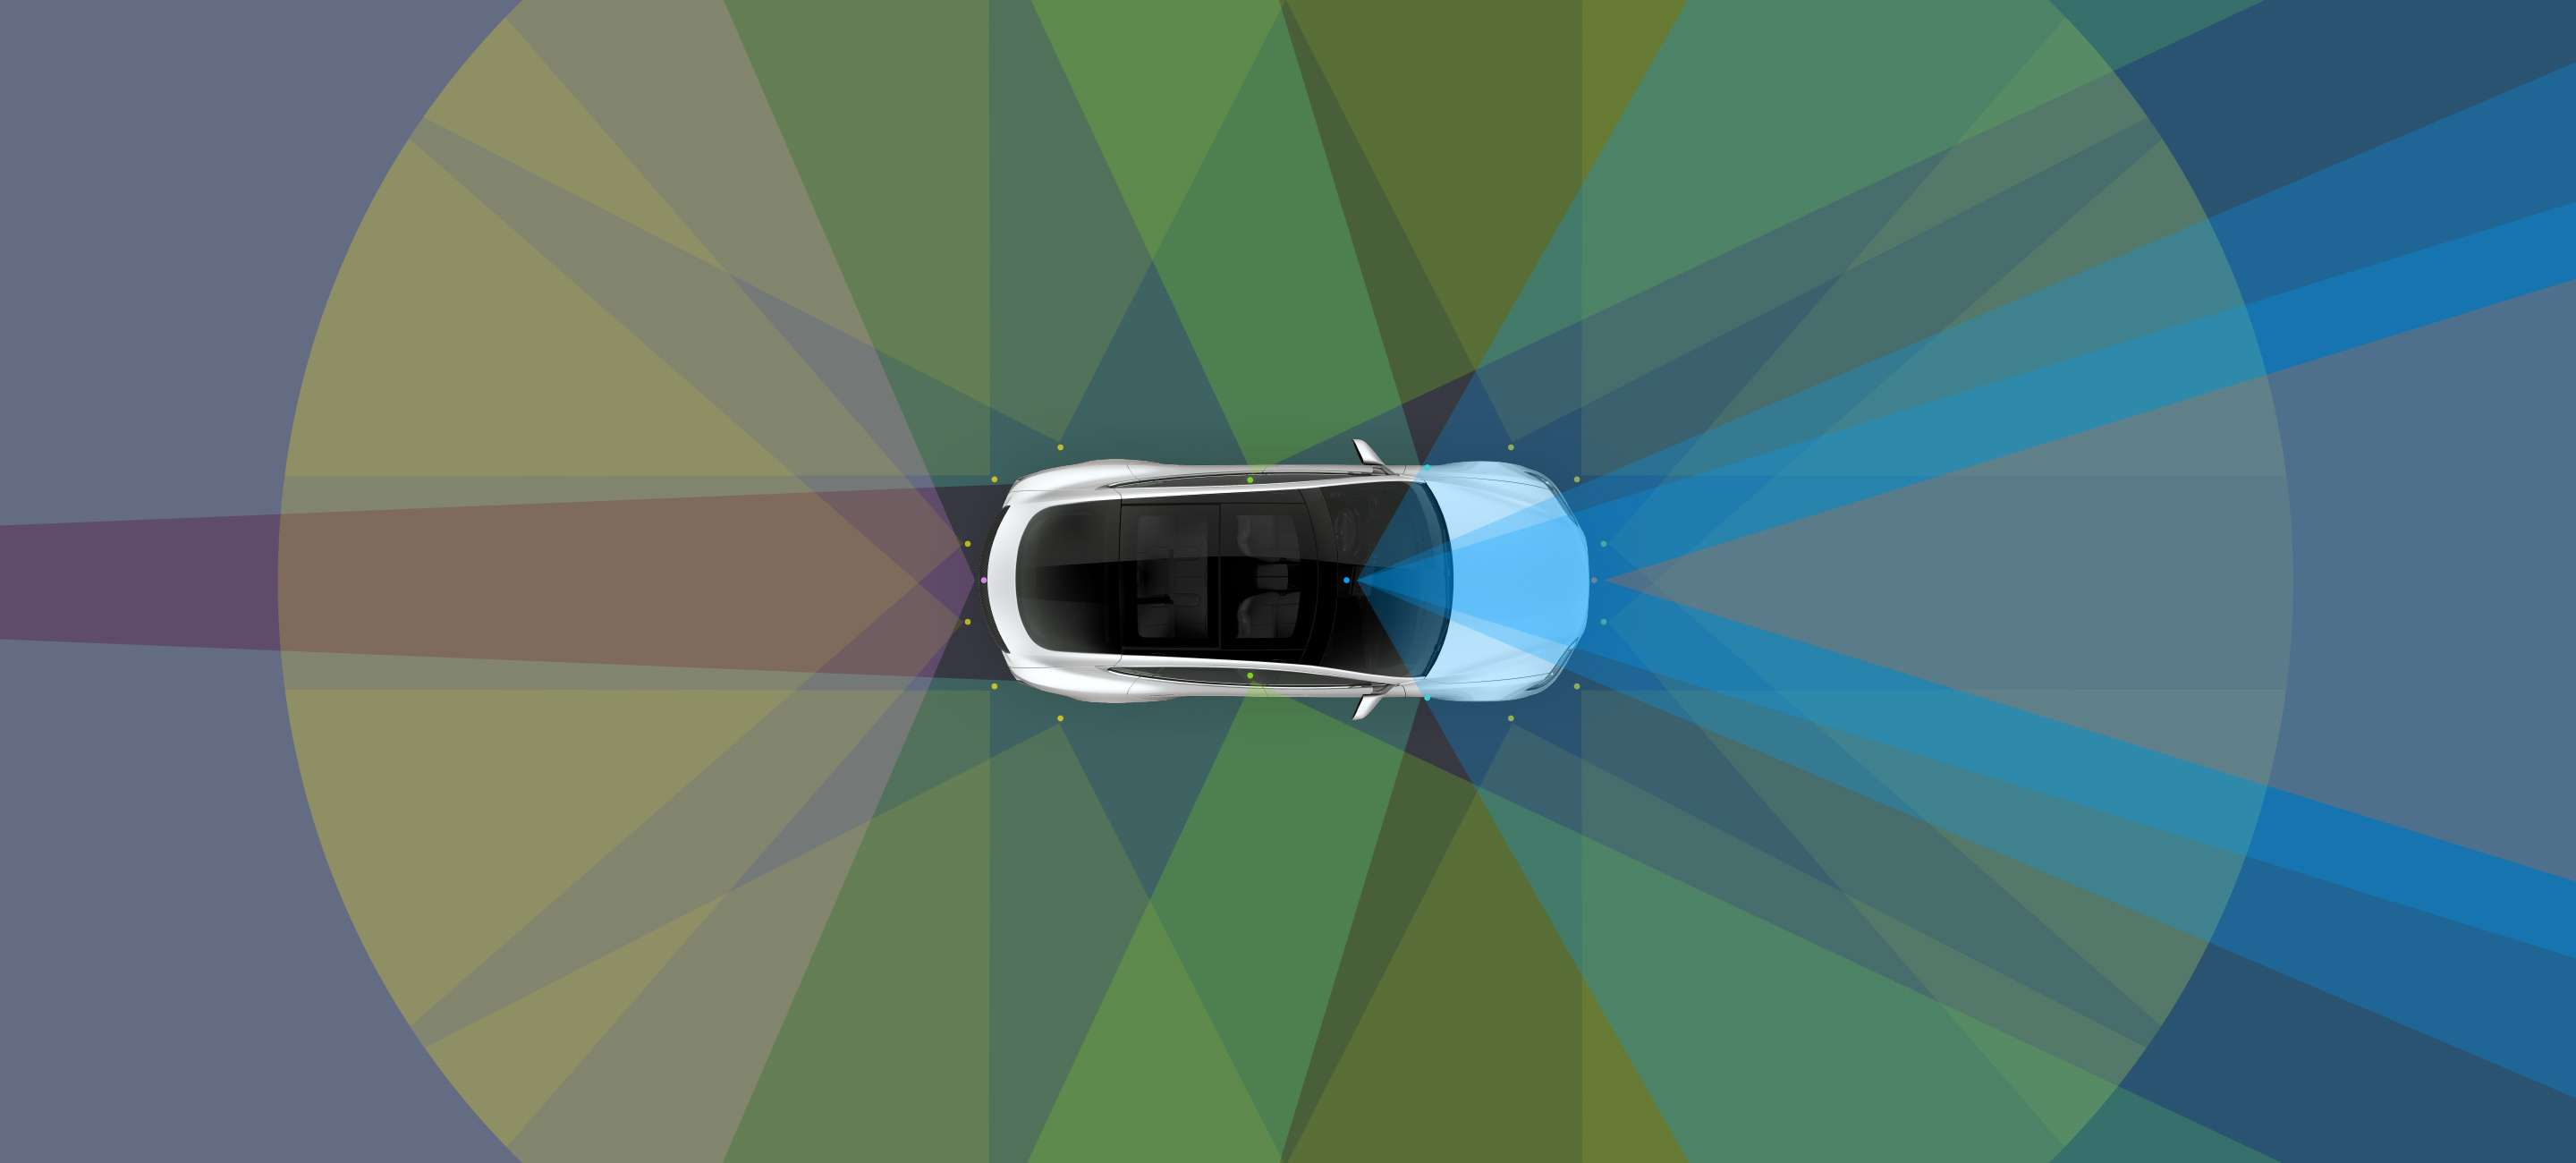
\includegraphics[width=\textwidth]{images/autopilotnew.jpg} 
\end{center}

\begin{center}
\dots aber wenn wir nicht aufpassen kann es Probleme geben!
\end{center}
\end{frame}

%------------------------------------------------------------------------------------

\section{Was ist Maschinelles Lernen?}

\begin{frame}
\begin{center}
\huge
Wie funktioniert\\Maschinelles Lernen?
\end{center}
\end{frame}

\begin{frame}
\begin{center}
\Large Imitation - Mehr als nur Anerkennung!
\medskip\medskip

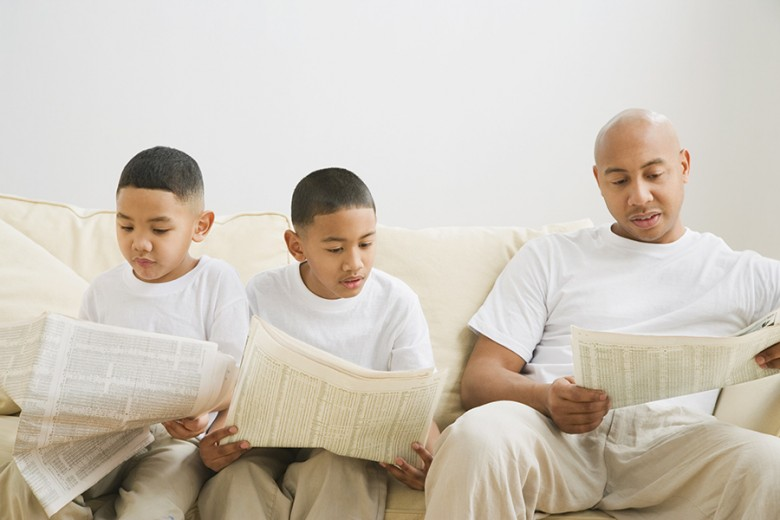
\includegraphics[scale=0.35]{images/imitation}
\end{center}
\end{frame}

\begin{frame}
\begin{center}
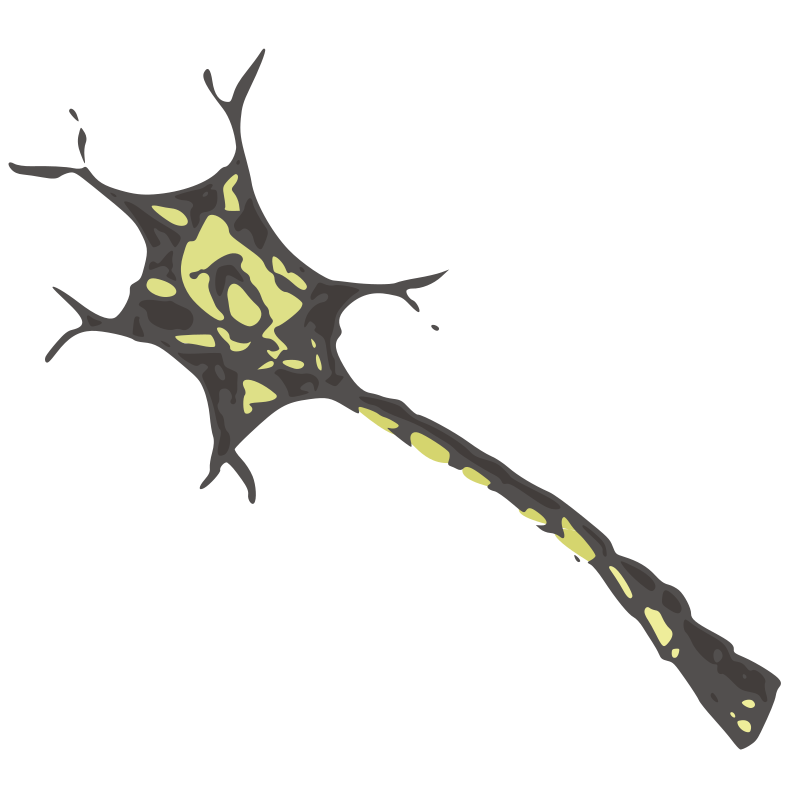
\includegraphics[height=0.8\textheight,keepaspectratio]{images/neuron} 
\end{center}
\end{frame}

\begin{frame}
\begin{center}
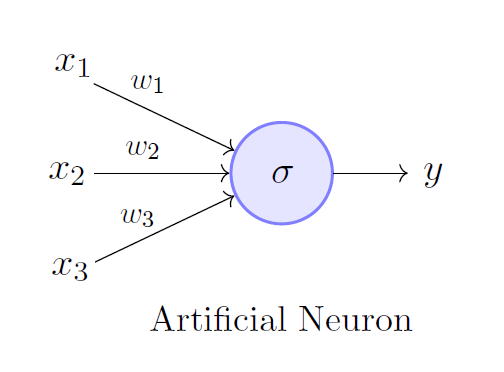
\includegraphics[height=.9\textheight,keepaspectratio]{images/perceptron} 
\end{center}
\end{frame}

\begin{frame}
\begin{center}
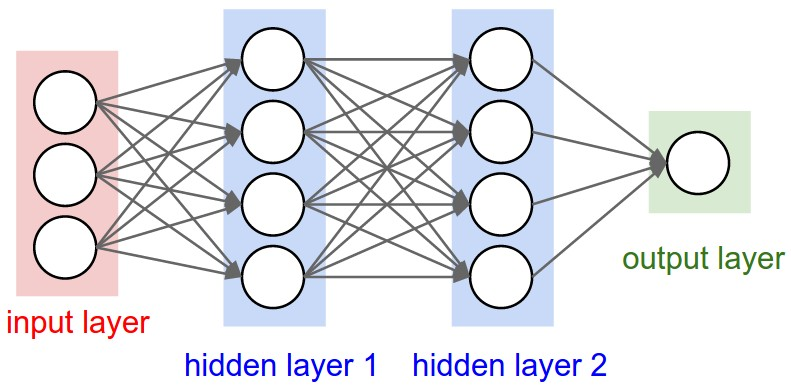
\includegraphics[width=\textwidth]{images/simple_neural_network_header.jpg} 
\end{center}
\end{frame}

\begin{frame}
\begin{center}
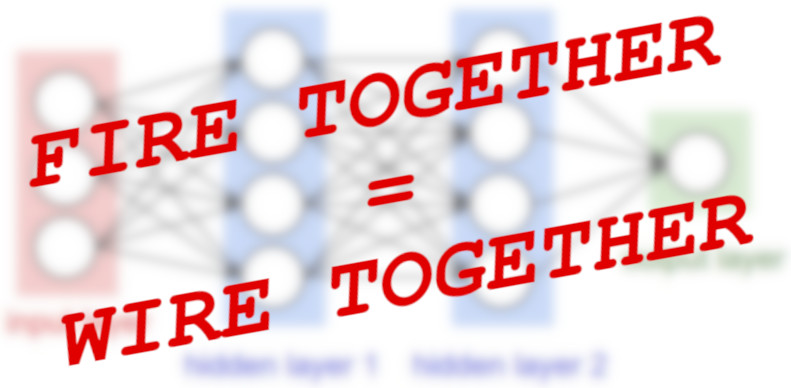
\includegraphics[width=\textwidth]{images/simple_neural_network_header_FW.jpg} 
\end{center}
\end{frame}

%------------------------------------------------------------------------------------

\section{Die Probleme}

%------------------------------------------------------------------------------------

\subsection{Common Problems}

\begin{frame}
\begin{center}
\Huge
\textbf{Probleme} \bigskip

\huge \textit{Theorie und Praxis}
\end{center}
\end{frame}

\begin{frame}[fragile]

\begin{center}
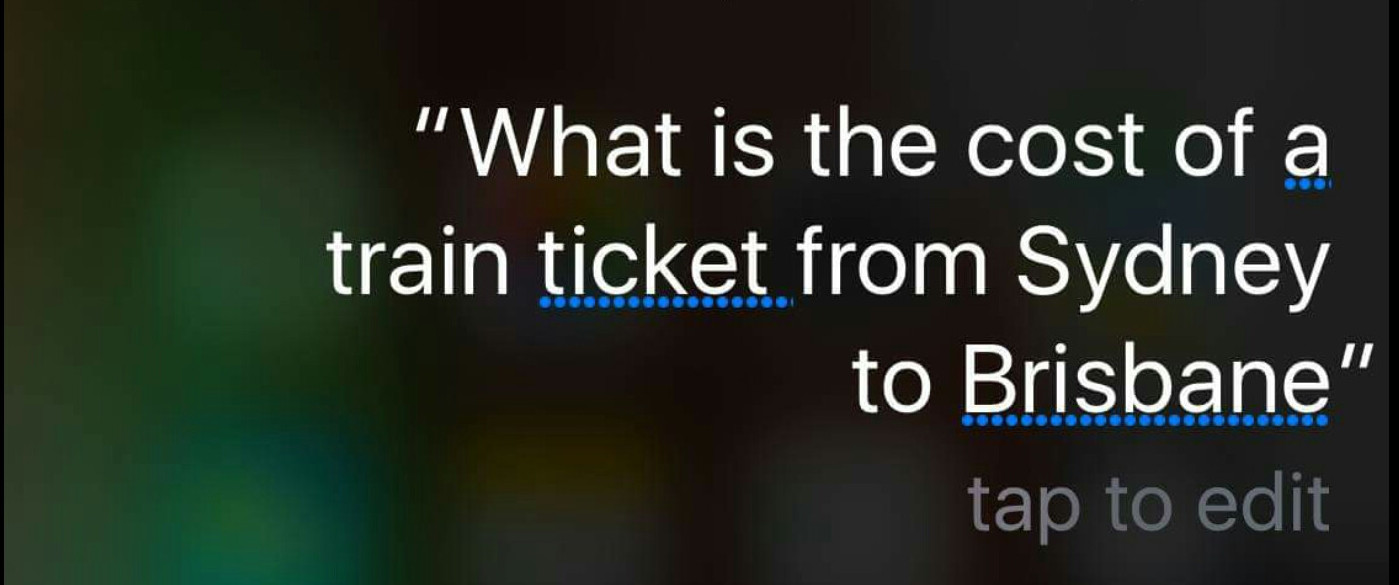
\includegraphics[scale=0.125]{images/sirifail1.jpg} 
\end{center}

\pause

\begin{multicols}{2}

\begin{center}
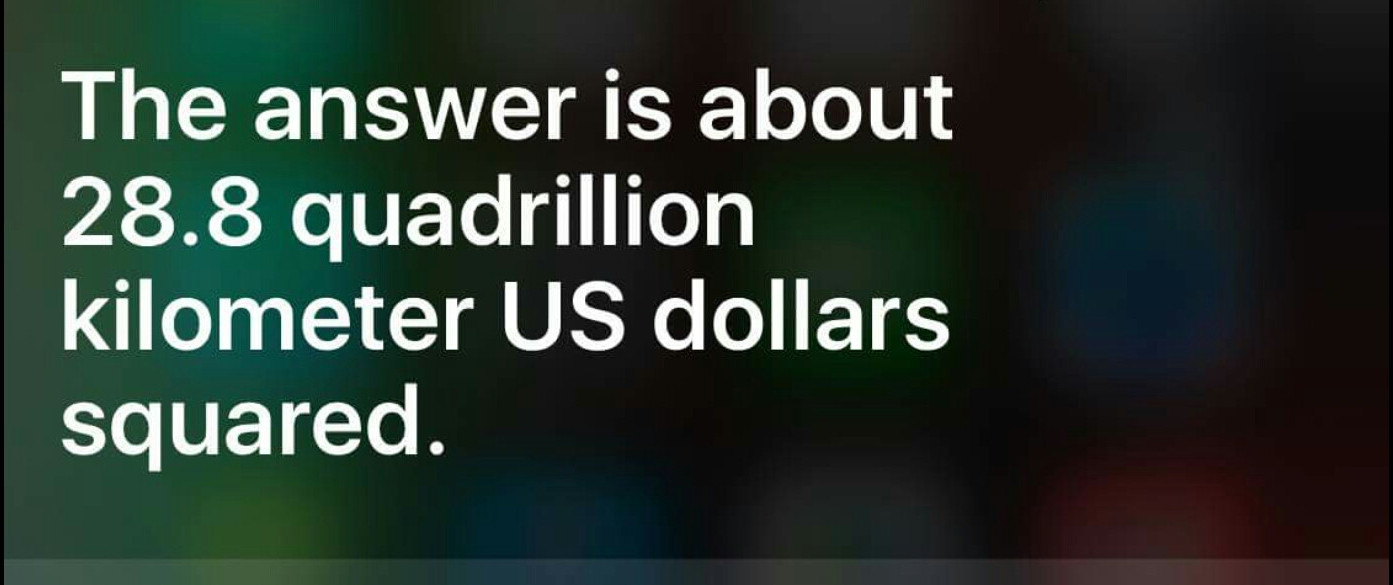
\includegraphics[scale=0.11]{images/sirifail2.jpg} 
\end{center}

\columnbreak
\pause

\begin{center}
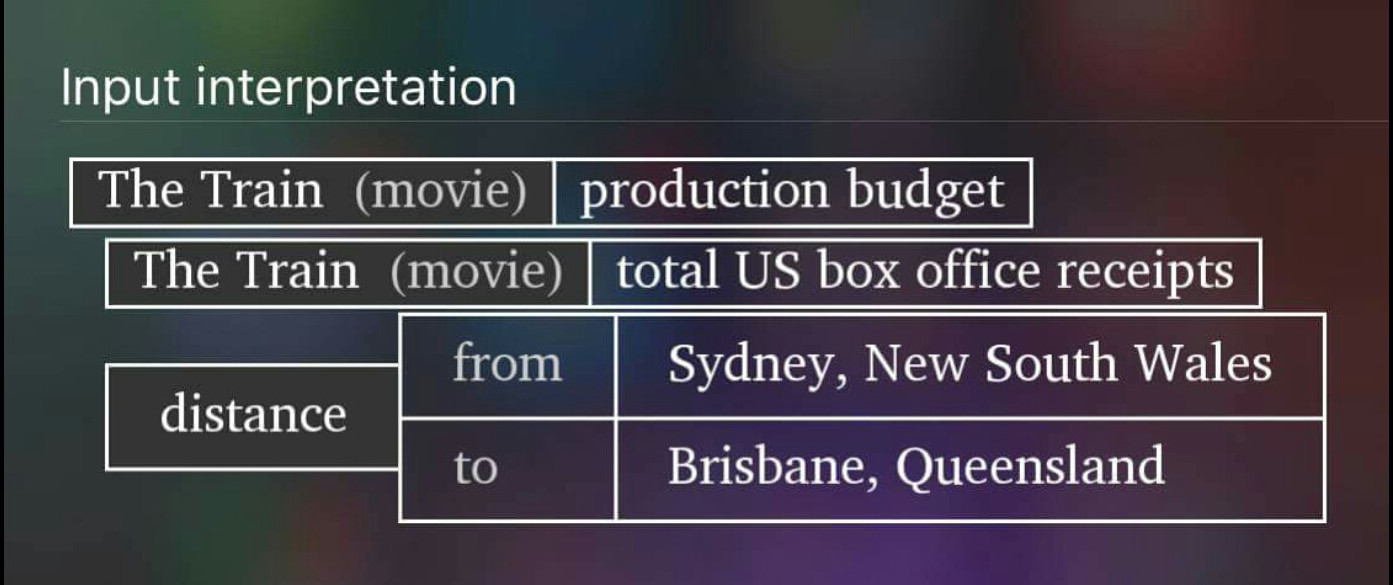
\includegraphics[scale=0.11]{images/sirifail3.jpg} 
\end{center}

\pause
\Put(-200,50){
\includegraphics[scale=1.5]{images/manshrug.png}}

\end{multicols}
\end{frame}

\begin{frame}
\begin{center}
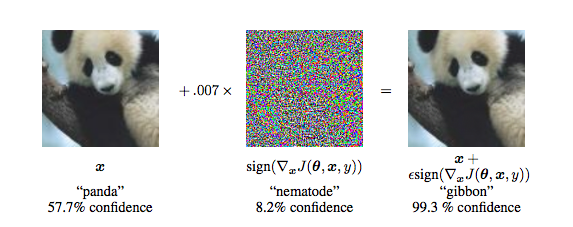
\includegraphics[width=\textwidth,keepaspectratio]{images/recog_panda.png} 
\end{center}
\end{frame}

\begin{frame}
\begin{center}
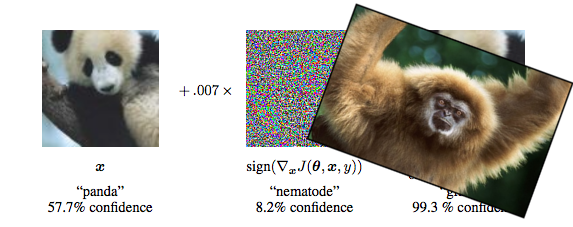
\includegraphics[width=\textwidth, keepaspectratio]{images/recog_gibbon.png} 
\end{center}

\pause
\Put(-40,0){
\includegraphics[scale=1.5]{images/manshrug.png}}
\end{frame}

\begin{frame}
\begin{center}
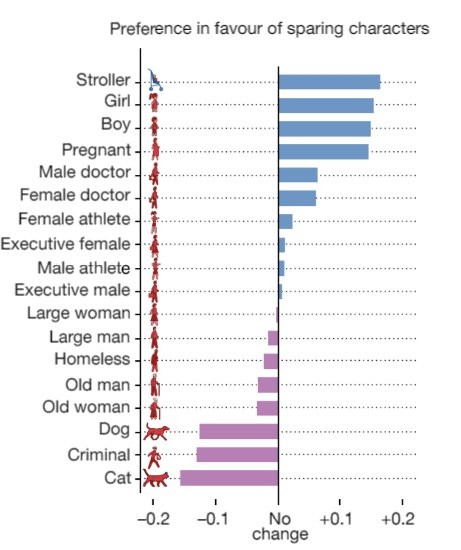
\includegraphics[height=0.9\textheight,keepaspectratio]{images/sparing} 
\end{center}
\pause
\Put(220,110){
\includegraphics[scale=1.5]{images/manshrug_rotate.png}}
\end{frame}

%------------------------------------------------------------------------------------

\subsection{Adversarial Objects}
\begin{frame}
\begin{center}
\huge
\glqq Adversarial Objects\grqq \\
\Large
(Feindliche Objekte)
\end{center}
\bigskip
\normalsize

(\textit{Subs., plural}) Objekte, die für das menschliche Auge herkömmlich erscheinen, aber für den Computer radikal anders aussehen.
\bigskip

\begin{center}
\textbf{Quelle:}\\
\emph{Fooling Neural Networks in the Physical World}\\
\url{https://www.labsix.org/}
\end{center}
\end{frame}

\begin{frame}
\begin{center}
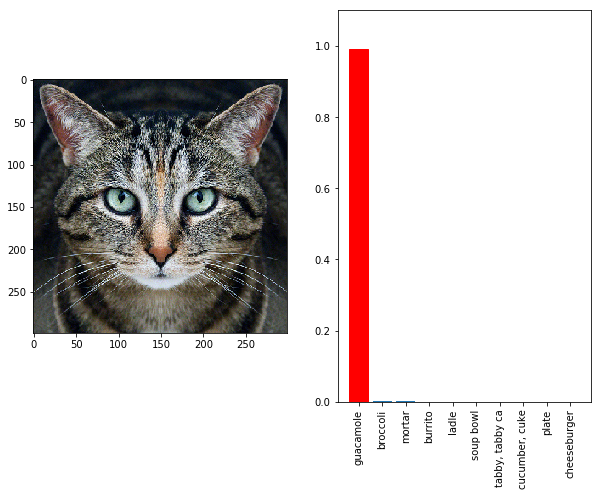
\includegraphics[height=0.95\textheight,keepaspectratio]{images/cat_adversarial.png} 
\end{center}
\end{frame}

\begin{frame}
\begin{center}
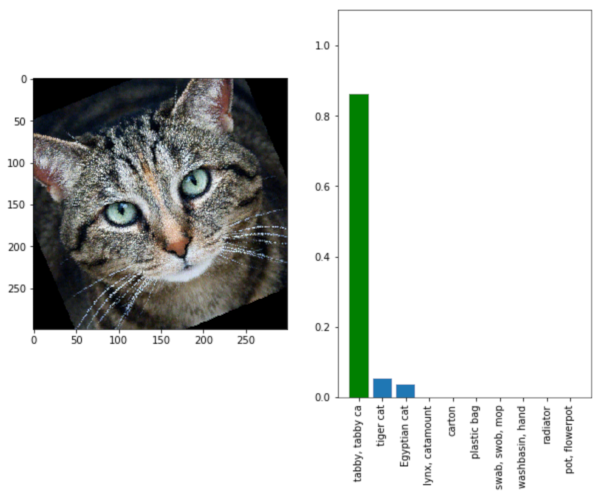
\includegraphics[height=0.95\textheight,keepaspectratio]{images/cat_rotated.png} 
\end{center}
\end{frame}

\begin{frame}

\begin{center}
Feindliche 3D-gedruckte Schildkröte:
\end{center}

\begin{center}
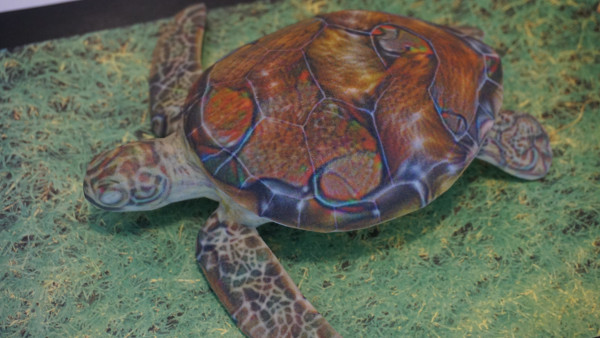
\includegraphics[height=0.7\textheight,keepaspectratio]{images/rifle_turtle.jpg} 
\end{center}
\end{frame}

\begin{frame}
\begin{center}
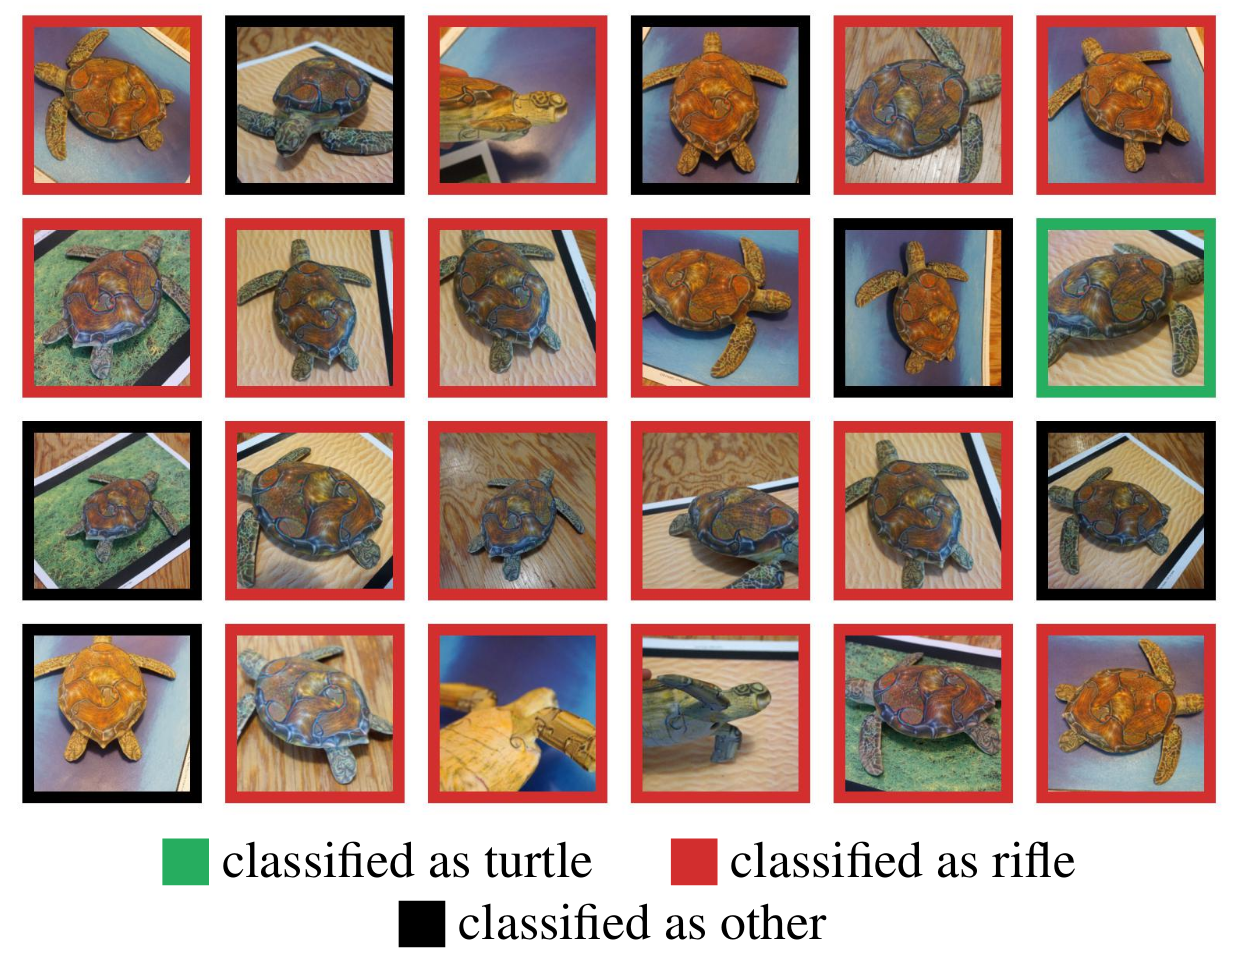
\includegraphics[height=0.9\textheight,keepaspectratio]{images/turtle_class} 
\end{center}
\end{frame}

\begin{frame}
\begin{center}
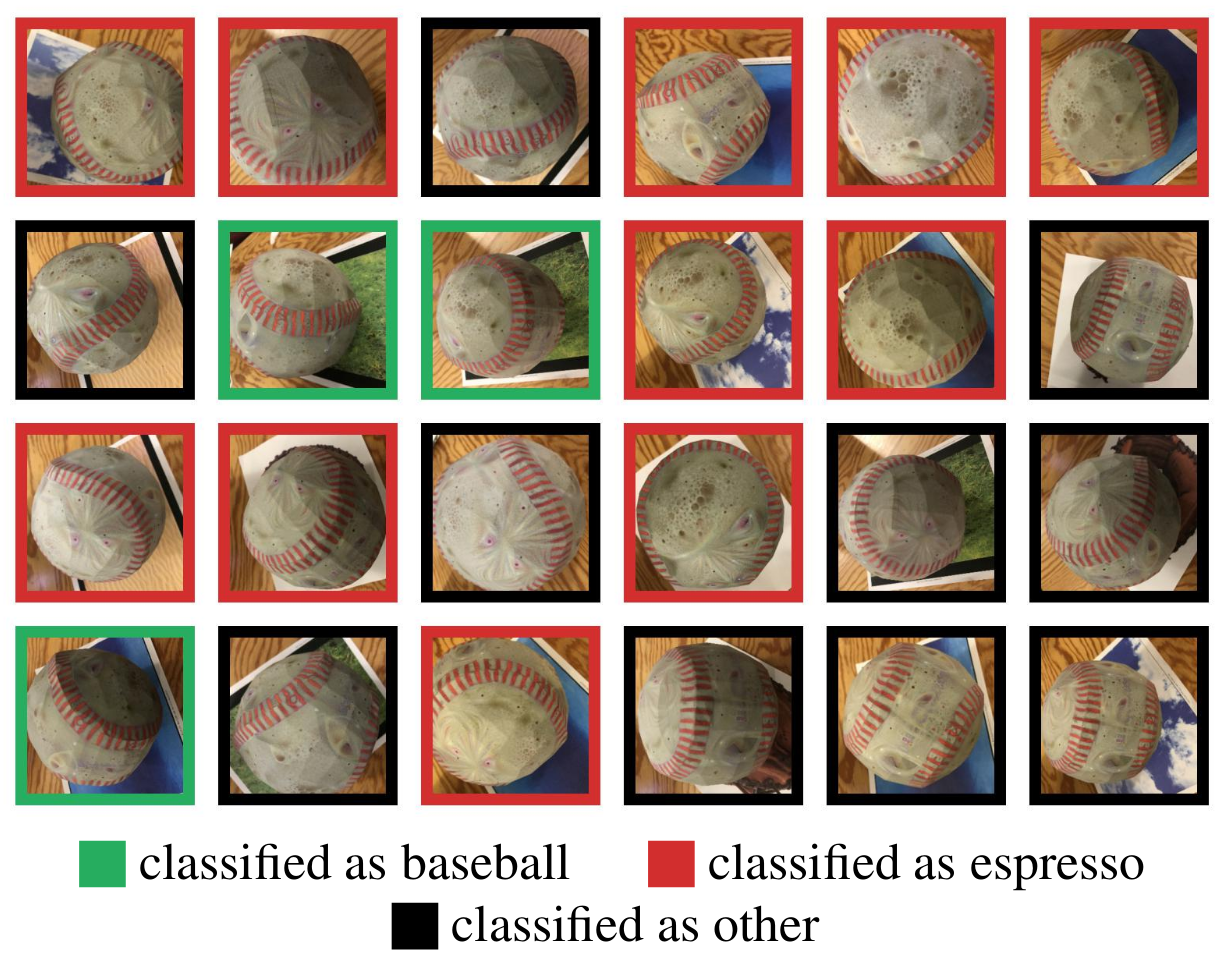
\includegraphics[height=0.9\textheight,keepaspectratio]{images/baseball_class} 
\end{center}
\end{frame}

\begin{frame}[fragile]

\begin{multicols}{2}

\vspace*{73pt}

\includegraphics[scale=0.6]{images/Happy-Thumbs-Up-Robot.png} 

\columnbreak

\vspace*{40pt}

\Huge
\hspace*{-30pt}Vielen Dank\\ für's\\ Zuhören!
\end{multicols}
\end{frame}

\end{document}

